\chapter{Équations différentielles à coefficients constants\label{annexe-eqndiff}}
\chaptermark{Équations différentielles}

\section{Définition}
La forme la plus générale d'une équation différentielles à coefficients constants est donnée
par :
\begin{align}
\sum_{i=0}^{n}a_i\devi{s(t)}{i}=\sum_{i=0}^{m}b_i\devi{e(t)}{i}
\end{align}


\section{Résolution équation différentielle du premier ordre}

La forme générale d'une équation différentielle du premier ordre est
donnée par : 
$$
a_1\devi{s(t)}{}+a_0s(t)=e(t)
$$
Il est toujours possible de simplifier une telle équation sous la forme :
$$
\devi{s(t)}{}+\dfrac{a_0}{a_1}s(t)=e(t)
$$


\subsection{Sans second membre}
$$
a_1\devi{s(t)}{}+a_0s(t)=0
$$

La solution générale de l'équation sans second membre est de la forme :
$$
s(t) = C e^{-\frac{a_0}{a_1}t}\,\,\,\,\text{avec}\,\,\,\,C\in\mathbb{R}
$$

On considère l'équation différentielle suivante régissant l'entrée                                                                        
et la sortie d'un SLCI\footnote{Système Linéaire Continu et Invariant} :                                                                  
$$                                                                                                                                        
\devi{s(t)}{}+as(t)=be(t)                                                                                                                 
$$                                                                                                                                        
avec pour condition initiale $s(0)=s_0$.                                                                                                  
On cherche à déterminer la réponse indicielle de ce système.                                                                              
                                                                                                                                          
\question{}                                                                                                                               
\textbf{Déterminer la réponse libre du système (sans second membre).}                                                                     
                                                                                                                                          
La réponse libre du système $s_1(t)$ satisfait l'équation différentielle                                                                  
$$                                                                                                                                        
\devi{s_1(t)}{}=-as_1(t)                                                                                                                  
$$                                                                                                                                        
Cette réponse ne dépend que des conditions initiales, ici $s(0)=s_0$.                                                                     
Cette solution est donc de la forme :                                                                                                     
$$                                                                                                                                        
s_1(t)=Ce^{-at}                                                                                                                           
$$                                                                                                                                        
avec $C$ une constante réel. La réponse doit satisfaire la condition initiale $s(0)=s_0$.                                                 
Ce qui impose :                                                                                                                           
$$                                                                                                                                        
s_1(t)=s_0e^{-at}                                                                                                                         
$$                                                                                                                                        
                                                                                                                                          
\question{}                                                                                                                               
                                                                                                                                          
\textbf{Déterminer une solution particulière de l'équation avec second membre par                                                         
la méthode de la variation de la constante.}                                                                                              
                                                                                                                                          
La réponse indicielle est donnée pour $e(t)=u(t)$. Pour $t>0$, l'équation différentielle                                                  
avec second membre est alors :                                                                                                            
$$                                                                                                                                        
\devi{s(t)}{}+as(t)=b                                                                                                                     
$$                                                                                                                                        
                                                                                                                                          
Déterminons une solution particulière $s_2(t)$ de cette                                                                                   
équation différentielle de la forme :                                                                                                     
$$                                                                                                                                        
s_2(t)=\lambda(t)e^{-at}.                                                                                                                 
$$                                                                                                                                        
En introduisant, celle-ci dans l'équation différentielle on a alors :                                                                     
$$                                                                                                                                        
\lambda'(t)e^{-at}-a\lambda(t)e^{-at}+a\lambda(t)e^{-at}=b                                                                                
$$                                                                                                                                        
On cherche une primitive de la dérivée de $\lambda$ à partir de :                                                                         
$$                                                                                                                                        
\lambda'(t)=be^{at}                                                                                                                       
$$                                                                                                                                        
soit alors :                                                                                                                              
$$                                                                                                                                        
\lambda(t)=\dfrac{b}{a}e^{at}+C                                                                                                           
$$                                                                                                                                        
avec $C$ une constante d'intégration.                                                                                                     
$$                                                                                                                                        
s_2(t)=\dfrac{b}{a}+Ce^{-at}.                                                                                                             
$$                                                                                                                                        
                                                                                                                                          
\question{}                                                                                                                               
\textbf{Donner la forme de la réponse totale. Tracer cette solution.}                                                                     
                                                                                                                                          
La solution générale est donnée par la somme des deux réponses précédentes:                                                               
\begin{align*}                                                                                                                            
    s(t)&=s_1(t)+s_2(t)\\                                                                                                                 
    s(t)&=s_0e^{-at}+\dfrac{b}{a}+Ce^{-at}                                                                                                
\end{align*}                                                                                                                              
La constante $C$ se détermine à partir de la condition initiale:                                                                          
$$                                                                                                                                        
s(t)=s_0e^{-at}+\dfrac{b}{a}\left(1-e^{-at}\right)                                                                                        
$$                                                                                                                                        
\begin{center}                                                                                                                            
        \begin{tikzpicture}                                                                                                               
                \begin{axis}                                                                                                              
                    [                                                                                                                     
                    height=7.5cm,                                                                                                         
                    width=10cm,                                                                                                           
                    grid=both,                                                                                                            
                    minor tick num=4,                                                                                                     
                    xmin=-1,                                                                                                              
                    xmax=12,                                                                                                              
                    ymin=-0.2,                                                                                                            
                    ymax=1.0,                                                                                                             
                    xlabel={$t$},                                                                                                         
                    ylabel={$s(t)$},                                                                                                      
                    clip=false                                                                                                            
                    ]                                                                                                                     
                    \addplot [very thick,color=blue,domain=-1:0, samples=101]{0};                                                         
                    \addplot [very thick,color=red,domain=0:12, samples=501]{  0.5*exp(-0.5*x)+0.5} node[above,xshift=-2em] {$s_0=1$};    
                    \addplot [very thick,color=blue,domain=0:12, samples=501]{-0.5*exp(-0.5*x)+0.5} node[below,xshift=-2em] {$s_0=0$};    
                    \draw[dashed] (axis cs:-1,0.5) node[left,xshift=-1em] {$\dfrac{b}{a}$}-- (axis cs: 12,0.5);                           
                \end{axis}                                                                                                                
        \end{tikzpicture}                                                                                                                 
\end{center}                                                                                                                              
                                                                                                                                          
\question{}                                                                                                                               
\textbf{En observant les différents termes de cette réponse,                                                                              
décomposer la solution en régime transitoire et régime permanent.}                                                                        
                                                                                                                                          
Sur les trois termes de la solution générale, un seul est non                                                                             
nul pour $t\to\infty$. Il correspond au régime permanent de                                                                               
la réponse. Les deux autres correspondent au régime transitoire.                                                                          
\begin{align*}                                                                                                                            
    s(t)=\textcolor{orange}{s_0e^{-at}-\dfrac{b}{a}e^{-at}}&+\textcolor{magenta}{\dfrac{b}{a}}\\                                          
    \textcolor{orange}{transitoire} &\quad\textcolor{magenta}{permanent}                                                                  
\end{align*}                                                                                                                              











































































































